% +---------------------------------------------------------------+
% | Author :    Noémie Plancherel, HEIG-VD
% | Date :      18.04.2022
% +---------------------------------------------------------------+

\chapter{Étude sécuritaire}
\label{ch:etude_secu}

Ce chapitre est dédié à toute l'analyse sécuritaire des gestionnaires de mots de passes en général. Nous allons dans un premier temps décrire comment ces applications sont sécurisées en fonction de leur type, puis justifier l'importance d'une forte sécurité suite à l'augmentation de la demande des entreprises et des particuliers.

Dans un second temps, nous allons identifier et analyser toutes les menaces existantes et / ou potentielles des \textit{password manager} en mettant en avant les failles actuellement connues des constructeurs et les conséquences de ces dernières ou des faiblesses qui pourraient survenir à tout moment (par exemple des cyberattaques).

Finalement, nous allons rédiger toutes les exigences sécuritaires que doivent respecter les gestionnaires de mots de passe afin que ces dernières garantissent une utilisation sûre qui évite des pertes ou vol de données.

\section{Implémentation de la sécurité dans les gestionnaires de mots de passe}

Dans cette section, afin de se baser sur des gestionnaires de mots de passe déjà existants et de pouvoir comparer les différentes sécurités implémentées, nous allons reprendre les 9 candidats sélectionnés dans la partie \hyperref[ch:etude_marche]{\textit{étude de marché}}, c'est-à-dire; \textit{LastPass}, \textit{Dashlane}, \textit{1Password}, \textit{KeePass}, \textit{Bitwarden}, \textit{NordPass}, \textit{Padloc}, \textit{Keeper} et \textit{Firefox}. Toutes les informations citées sont basées sur les \textit{security whitepapers} des constructeurs\cite{lastpasssecurity}\cite{dashlanesecurity}\cite{1passwordsecurity}\cite{keepasssecurity}\cite{bitwardensecurity}\cite{padlocsecurity}\cite{keepersecurity}.

Les gestionnaires de mots de passe sélectionnés fonctionnent tous de la même manière, au final cette méthode est plutôt classique dans les architectures des applications. Un \textit{master password} (qui est seulement connu par l'utilisateur) est généré ou entré par l'utilisateur et va permettre le déverrouillage de l'application et le chiffrement / déchiffrement en local de toutes les données stockées. 

À part pour les gestionnaires en local qui gèrent la sécurité différemment, ils mettent en avant le \textit{Zero-knowledge encryption}. C'est une méthode qui va permettre un chiffrement \textit{end-to-end} et qui va sécuriser au mieux les données personnelles et sensibles des utilisateurs, des serveurs du constructeur. En sachant que toutes les données sont stockées dans le cloud du provider, afin d'éviter que n'importe qui puisse y avoir accès, toutes les données sont chiffrées avant d'être envoyées au serveur. Ainsi, les données sont uniquement déchiffrées sur le device de l'utilisateur et la clé de chiffrement reste également en local.

Nous allons décrire dans les sous-sections suivantes comment la sécurité est implémentée dans les gestionnaires de mots de passe en fonction de leur type afin d'aller un peu plus en détail. 

\subsection{Les gestionnaires browser-based}
Les gestionnaires de mots de passe \textit{browser-based} proposent des fonctionnalités classiques et ne sont pas très poussés. Ce sont des applications légères qui sont pensées pour faciliter au mieux les utilisateurs.\cite{Browser}

Par défaut, ces applications n'activent pas de \textit{master password} et certaines n'en proposent même pas pour ajouter un chiffrement supplémentaire. Toutefois, ils proposent la fonctionnalité de 2FA.

Firefox fonctionne localement ou avec la synchronisation qui demande l'utilisation du cloud. Si la synchronisation n'est pas activée, les mots de passes stockés sont directement chiffrés sur l'appareil et sont ajoutés à un fichier \textit{logins.json} qui se trouve dans le répertoire de l'utilisateur. 

Il propose également la fonctionnalité d'ajouter un master password afin d'avoir une couche sécuritaire supplémentaire (par défaut, cette fonction est désactivée), ainsi, sans un mot de passe principal et sans l'activation du 2FA, les mots de passe sont accessibles en clair sur le navigateur dès le moment où on a accès à l'appareil et que l'utilisateur est connecté à son compte (ce qui est fortement probable, car le compte reste connecté, même après une fin de session). Toutefois, lors de l'ajout d'un master password, ce dernier est uniquement défini en local et n'est pas synchronisé entre profils ou appareils, mais il chiffrera toutes les données en local. 

Au niveau du fonctionnement\cite{firefoxEncr} (sans master password), les identifiants sont chiffrés à l'aide de 3DES-CBC et sont directement stockés dans un fichier JSON \textit{logins.json} encodés en ASN.1 puis en Base64. La clé de chiffrement est stockée dans une base de donnée \textit{key4.db}. Il existe actuellement des outils pour déchiffrer les mots de passe du gestionnaire.

Si l'option de synchronisation (\textit{Firefox Sync}) est activée\cite{firefoxsync}, les données stockées sur les serveurs Mozilla seront chiffrés. Nous pouvons se baser sur le schéma suivant qui explique le processus de synchronisation des données avec les serveurs Mozilla:
\begin{figure}[h!]
	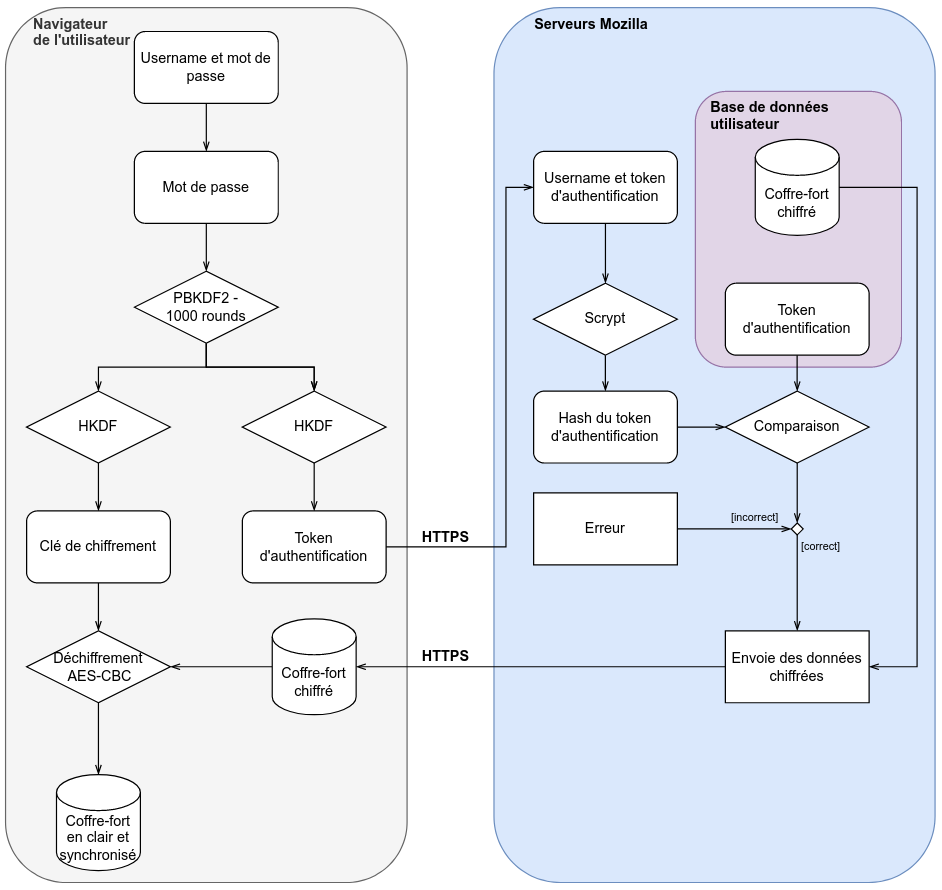
\includegraphics[width=15.5cm]{images/firefox_sync.png}
		\centering
	\caption{Schéma de synchronisation de données sur Firefox}
\end{figure}

Les données chiffrées sont protégées avec HMAC-SHA256 afin de pouvoir authentifier les données avant de les déchiffrer. La méthode utilisée est Encrypt-then-MAC. Cela permet de protéger l'intégrité des données en clair et chiffrées.

Comme cité précédemment, lors d'un ajout de master password afin de protéger les données localement, Firefox va tout d'abord chiffrer les données localement (le stockage se fait comme expliqué plus haut) et va les rechiffrer lors de la synchronisation avec le processus expliqué à l'aide du schéma.

Au final, ce design cryptographique est plutôt classique au sein des gestionnaires de mots de passe qui utilisent les serveurs du constructeur pour stocker les données.

Les autres gestionnaires de mots de passe browser-based fonctionnent en général de la même manière avec les données synchronisées. Chrome stocke également les identifiants dans un fichier local protégé avec DPAPI (Microsoft's Data Protection API).
\subsection{Les gestionnaires en local}
Pour les gestionnaires qui fonctionnent uniquement en local, nous allons nous baser sur l'implémentation sécuritaire de KeePass, qui est open-source, ce qui peut faciliter à comprendre tout le concept. Dans cette section, nous n'allons pas détailler toute l'architecture mais rester plutôt en surface. D'autres gestionnaires de mots de passe fonctionnent également en \textit{offline} avec un stockage local, cependant lors de la première connexion, il y a quand même des informations envoyées aux serveurs du constructeur (comme 1Password par exemple), ce qui n'est pas le cas pour l'application de base KeePass.

Etant donné que KeePass ne fonctionne qu'en local, il est important de bien gérer la mémoire et le stockage de données sensibles.

Toutes les données se trouvent dans un fichier de base de données spécial \textit{.kdbx}. Ce fichier contient toutes les données du gestionnaire (mots de passe, usernames, etc.) et est chiffré (également compressé en GZIP si on le souhaite). Dans la version de KeePass 2.x, les chiffrements supportés sont AES256-CBC et ChaCha20. 

La base de données est stockée où l'utilisateur le souhaite (avec une possibilité de la stocker dans un cloud), c'est pourquoi la sécurité repose sur la complexité du mot de passe. Elle est structurée avec un header et un contenu\cite{keepassstruct}\cite{keepassieee}.Dans le header, sont stockées différentes informations; un UUID indiquant le cipher, une indication si le fichier est compressé, différentes seed (voir \ref{schema_keepass}), l'IV pour le chiffrement et des bytes pour l'authentification (générés aléatoirement lors de la sauvegarde de la base de données). Le corps du fichier contient des blocs hachés avec HMAC-SHA256 et des blocs de données qui ont un format XML lorsqu'ils sont déchiffrés.

Tous les deux sont authentifiés avec le schéma Encrypt-then-Mac avec HMAC-SHA256. 

Au niveau de l'utilisation de la mémoire du processus, lors de l'ouverture de la base de données chiffrée, elle est chargée en mémoire. La protection de la mémoire s'applique aux données sensibles telles que la Master key et des mots de passe. Dès que la base de donnée est sauvegardée, les données chiffrées sont envoyées sur le disque.

 \newpage

\begin{wrapfigure}[28]{l}{0.55\textwidth} 
	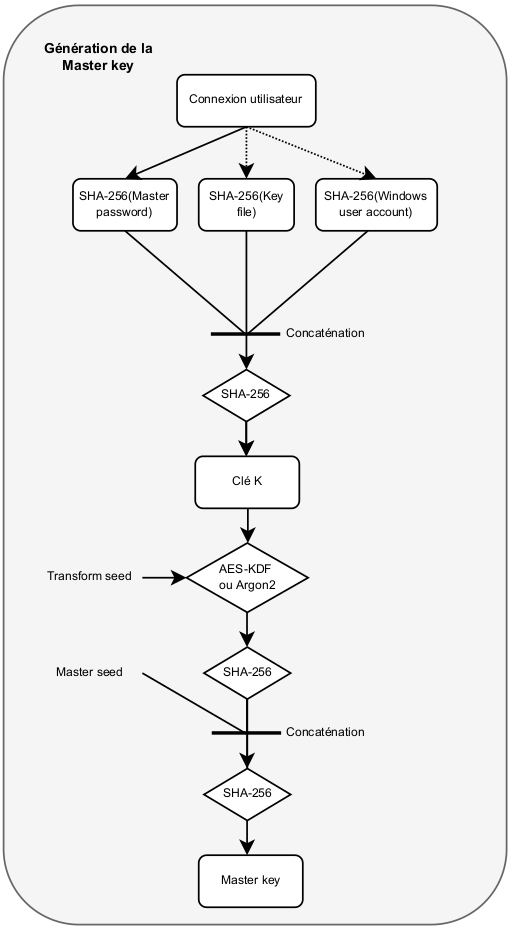
\includegraphics[width=0.5\textwidth]{images/keepass_generation_key.png}
	\caption{Génération de la Master key sur Keepass \label{schema_keepass}}
\end{wrapfigure}

La Master key sur KeePass prend plusieurs arguments différents et est générée d'une manière assez complexe. L'utilisateur doit obligatoirement fournir un master password, et peut également utiliser un key file et / ou le compte utilisateur Windows. 

Chaque composant est haché avec SHA-256 et sont concaténés et hachés ensemble. En output, on a une clé composite K qui va être dérivée à l'aide de AES-KDF ou Argon2. Les paramètres de ces deux algorithmes peuvent être configurés dans les paramètres de la base de données.

Chaque output est haché avec SHA-256 et au final, on obtient la Master key qui permettra de déchiffrer la base de données.

Les deux différentes seeds utilisées dans la génération de la clé sont stockées dans le header de la base de données \textit{.kdbx}.

Cette architecture permet de se protéger contre les attaques par dictionnaires et le brute-force de la Master key.

\subsection{Les gestionnaires cloud-based}
Les gestionnaires de mots de passes cloud-based ont tous une architecture similaire dû au fait que toutes les données sont stockées sur les serveurs du constructeur. Il y a des différences avec l'authentification de l'utilisateur et des algorithmes cryptographiques choisis, mais le design sécuritaire a la même base au niveau de la connexion de l'utilisateur et du chiffrement du gestionnaire. 

Ainsi, afin d'expliquer un peu plus en détail le fonctionnement d'un gestionnaire cloud-based, nous allons prendre l'exemple de LastPass. Nous allons nous basé sur le schéma ci-dessous afin d'appuyer nos propos.
\begin{figure}[h!]
	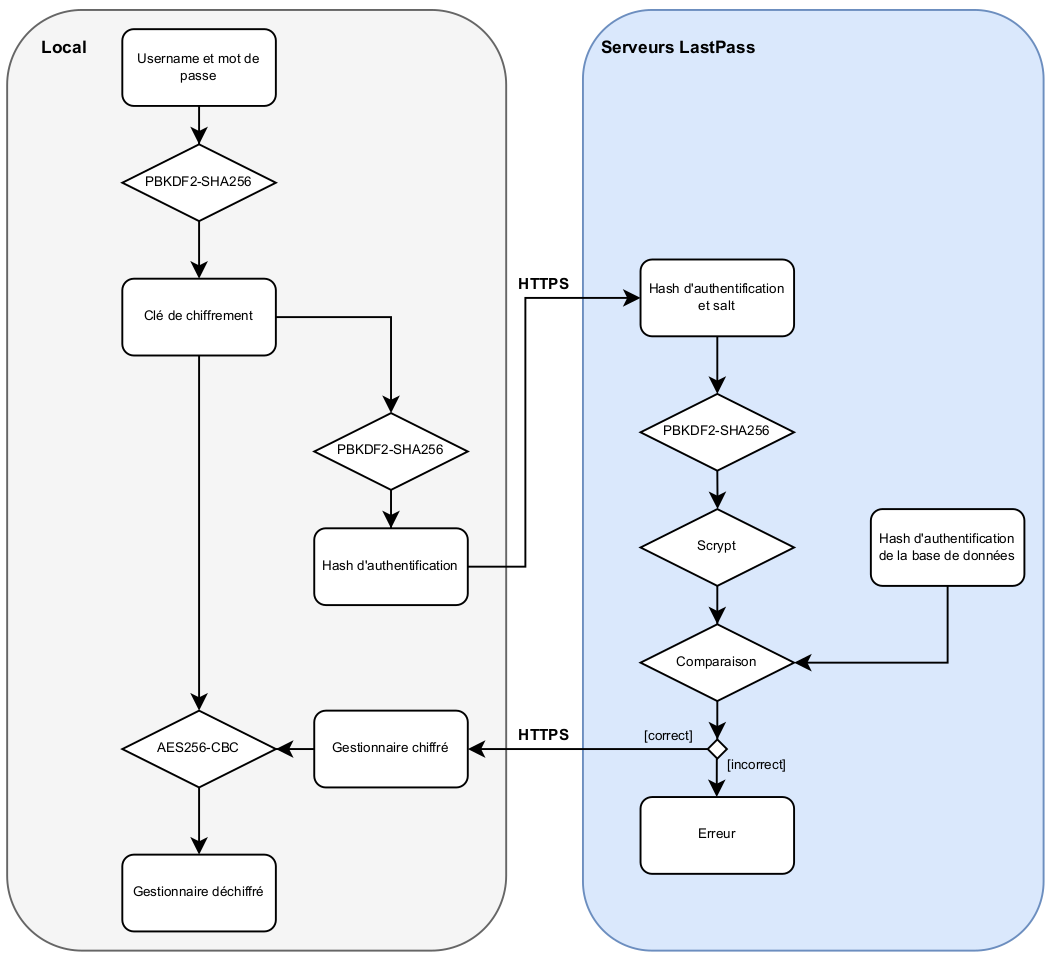
\includegraphics[width=15.5cm]{images/lastpass_encr.png}
	\centering
	\caption{Schéma de déchiffrement de LastPass}
\end{figure}

Afin de générer la clé de chiffrement, ce dernier dérive le master password en utilisant le nom d'utilisateur comme sel. Il utilise l'algorithme PBKDF2-SHA256 avec 100'100 rounds. 
\subsection{Partage d'informations}
\subsection{Perte du master password}
\subsection{3 états du gestionnaire de mot de passe}
Les gestionnaires de mots de passe ont généralement 3 états différents, \textit{Not Running}, \textit{Unlocked State} et \textit{Locked State}. Nous allons expliquer plus en détails comment ils fonctionnent lorsqu'ils sont dans les différents états. Nous nous basons sur un article qui analyse le management des secrets\cite{iseexploit}.
\subsubsection{Etat \textit{Not Running}}
C'est l'état du password manager lorsqu'il n'a jamais été utilisé et configuré après son installation. On définit également cet état s'il n'a pas été lancé depuis le dernier redémarrage du système ou a été arrêté par un utilisateur. Dans cet état, le gestionnaire doit garantir qu'il n'y a aucune donnée sensible stockée sur le disque, comme une clé de chiffrement ou le master password.
\subsubsection{Etat \textit{Unlocked State}}
Cet état indique que le gestionnaire fonctionne et donc, l'utilisateur a entré son master password afin de déchiffrer toutes les données afin d'avoir accès aux informations stockées. Le gestionnaire doit garantir qu'il n'est pas possible d'extraire aucune information sensible de la mémoire.
\subsubsection{Etat \textit{Locked State}}
Nous considérons cet état lorsque l'utilisateur a lancé le gestionnaire (déjà configuré) sans avoir encore entré le master password ou qu'il a lui même verrouiller son gestionnaire. À ce moment, il ne devrait pas y avoir de données sensibles stockées sur le disque afin d'éviter toute extraction. 
\subsection{Algorithmes cryptographiques}
- les algos utilisés pour le chiffrement et auth des données 
\subsection{L'importance d'une forte sécurité}
\colorbox{pink}{\parbox{15cm}{à voir si utile}}
\section{Analyse des menaces}
\subsection{Failles connues des constructeurs}
\colorbox{pink}{\parbox{15cm}{à voir si je devrais pas les ajouter dans le chapitre de l'analyse de chaque gestionnaire sélectionné}}
\subsection{Conséquences d'une quelconque faiblesse}
\colorbox{pink}{\parbox{15cm}{à voir si utile, mais les conséquences seront sûrement soulignées lorsque je ferai l'analyse de menaces de toute manière}}
- remember me du master password HAA
\section{Exigences sécuritaires à respecter}